\documentclass[12pt]{article}

\usepackage[utf8]{inputenc}
\usepackage[english]{babel}
\usepackage{natbib}
\usepackage[T1]{fontenc}
\usepackage{setspace}
\usepackage{graphicx}
\usepackage{hyperref}
\usepackage{float}
\usepackage[top=3.5cm,left=2.7cm,right=2.7cm,bottom=3.5cm]{geometry} % 'showframe' to see borders
\usepackage{booktabs}

\graphicspath{ {diagrams/} }

\title{\vspace{2cm}6G6Z1705\\\textbf{Artificial Intelligence}\\\vspace{2cm}Scenario 2\\\vspace{2cm}}
\author{14032908\\Joshua Michael Ephraim Bridge\\joshua.m.bridge@stu.mmu.ac.uk\\\vspace{1cm}}

% \pagestyle{headings}

\begin{document}

\maketitle

\newpage

\doublespacing

\section{Introduction}
  In this report an AI classifier will be put forward which maps mamographical data to desired outputs (diagnoses). In order to do this two types of AI classifiers will be evaluated on their performance in this task, along with relevant pre-processing of the attributes to enhance classifier performance. The two classifier types will be a Decision Tree (J.48) and an Artificial Neural Network (Multilayer Perceptron, \cite{minsky2017perceptrons}). In order to evaluate their performance, considerations of both learning time \& classification accuracy will be taken into account.

\section{AI classifiers}
  In this section a brief study will be conducted into the two classifier types mentioned previously.

  \subsection{Decision Trees}
    A decision tree is a type of classifier (specifically a hierarchical variant of a multistage classifier, as defined by \cite{safavian1991survey}) which uses a tree-like structure to test values on different attributes in a format similar to a flow chart. The tree structure itself could be described as a single root node with 0 to many connected children, each themselves with 0 to many connected children. Any node in a decision tree with no children is known as a leaf node and has a direct relationship with a class label. At each node in the tree a test is carried out on an attribute and the result of that test decides on which of the child nodes the process should continue onto. The process of completing each test from the root node to a leaf node should result in a classification of the data provided.

    Self-learning decision trees are often very useful because they explicitly define how the instances are classified within the tree, simplifying the process into a set of simple rules. This is different to ANN's (see section \ref{ann}) where the classification process is mostly hidden and can often be a very complex set of rules which would be very hard to follow.

    \subsubsection{C4.5 Decision tree}
      There are several parameters within the C4.5 algorithm that will affect the classification performance on a dataset.

      % \paragraph{ID3}
      % \begin{equation} \label{eq:entropy}
      %   H(X) = -\sum p(X)\log p(X)
      % \end{equation}
      %
      %
      % \begin{equation} \label{eq:informationgain}
      %   I(X,Y)= H(X)-H(X|Y)
      % \end{equation}

      \paragraph{Confidence}
        The confidence parameter is a way of controlling the amount of error-based pruning \citep{quinlan1987simplifying} within the decision tree. More specifically, post-pruning is the process of estimating the error rate (probability of mis-classification) at each node in the tree, and deciding whether or not to remove the node. Lower values of the confidence factor will result in the post-pruning becoming much more aggressive with removing nodes \citep{beck2008backward}.

      \paragraph{Minimum number of objects}
        Within weka the Minimum number of objects parameter controls the Minimum number of instances per leaf. This means that each leaf within the tree must have at least the specified amount of classified instances for it not to be pruned. This parameter is good for data-sets which are particularly noisy which could introduce some leaf nodes which are not very stable classifiers. With a higher minimum number of objects, the tree will likely become much more pruned.

    % https://www.ncbi.nlm.nih.gov/pmc/articles/PMC4466856/
    % https://medium.com/@mohtedibf/indepth-parameter-tuning-for-decision-tree-6753118a03c3

  % • A detailed description of decision tree parameters (individual research required) and how they might affect the performance of the classifier

  \subsection{Artificial Neural Networks} \label{ann}
    An Artificial Neural Network is a mathematical system which is able to classify data by performing a series of mathematical functions (activation functions) which take weightings for each of their inputs and summise them into a single output. ANN's are designed in light of the way human/animal brains process information, via a series of neurons which are connected (in biology these connections are called synapses). Within an ANN each neuron is connected to either input attributes or the output of neruron(s) in another layer of the network. The connections between the neurons contain weightings which is the main principal behind how the network can emphasise some data over others.

    The neurons within an ANN can be split up into a series of ‘layers’, where the outputs from one layer of neurons will become the inputs for the next layer of neurons. Within a Multilayer Perceptron (see section \ref{mlp}) the layers consist of 1 input layer, 1 output layer, and at least 1 ‘hidden layer’ where each neuron in the hidden layer(s) and the output layer are neurons which perform an activation function.

    Within an ANN there must be a process of ‘learning’ which enables it to find the most optimal values for the weights which are used in the activation functions. This is done via backpropagation which enables the algorithm to modify the weights based on the error rate of the output, compared to the expected output.

    % Learning occurs in the perceptron by changing connection weights after each piece of data is processed, based on the amount of error in the output compared to the expected result. This is an example of supervised learning, and is carried out through backpropagation, a generalization of the least mean squares algorithm in the linear perceptron.

      \subsubsection{Multilayer Perceptron} \label{mlp}
        \citep{minsky2017perceptrons}
        \paragraph{Hidden Layers}
          The hidden layers parameter allows the user to define the strcuture of the network they would like to train. Introducing more layers \& neurons introduces more complexity which is good for more complex datasets with attributes which are not lineraly seperable, however for simpler datasets this may introduce unwanted complexity within the network. What hidden layers are and how they relate to the ANN is explained in more deatail in section \ref{ann}.

        \paragraph{Learning Rate}
          Learning rate applies to the backpropagation algorithm and more specifically the Gradient Descent. It concerns the speed at which the minimum squared error is reached. A low learning rate would mean that many updates (a high training time) would be needed in order to find the global minimum - which is not desirable. If the learning rate is too high however, then this can lead to divergent behaviour where the backpropagation algorithm is not able to correctly settle on an optimal minimum.

          % This algorithm aims at learning the weights of a multilayer ANN with a fixed number of units and interconnections, by using gradient descent in order to minimize the squared error between the network outputs and the correspondent target values.

          % The backpropagation algorithm can be viewed as a searching algorithm whose state space corresponds to all possible weights for the network units. The algorithm uses the squared error between the network outputs and the target values as a fitness function to guide the gradient descend. The correspondent error surface can thus be considered multidimensional and may have multiple local minima. This characteristic guarantees only that the gradient descent will converge to a local minima and not necessarily to the global minimum error.

        \paragraph{Momentum}
          Once again momentum relates to the gradient descent for squared error, however momentum defines the way in which the minima is reached. As there may be several local minimas within the descent path, it would not be desirable to end in a minima which is not actually the global minima. In order to avoid this, the momentum value is linked to the learning rate in that increasing the momentum allows the descent path to continue past local minimas in search of lower squared errors.
          % A descent gradient is used in order to reach the global minima. However, as this is trying to be found, the algorithm may encounter a local minimum which it may think is the global minima. This can be avoided by changing the value of the momentum, this parameter is linked to the learning rate so as momentum increases, learning rate should remain a smaller value to avoid the global minima from being missed.

        \paragraph{Training Time}
          The main factor in the learning process of an ANN is the amount of time it has to train. There is no point in time which the network will be ‘done’ learning, so the most optimal amount of learning time must be chosen.

\section{Data set analysis}
  % • Description of the data set attributes (e.g.):
  %   (a) Distribution,
  %   (b) predictive, (individual research required)
  %   (c) Outliers,
  %   (d) Attribute measurement scales e.g. nominal, ratio etc.

\section{Classifier Prediction}
  % • Based on the evidence from sections 2 and 3, what are the strengths and weaknesses of a decision tree when applied to the dataset

  % • Based on the evidence from sections 2 and 3, what are the strengths and weaknesses of an artificial neural network when applied to the dataset

  % • Prediction: which classifier is likely to be best for the dataset (before you have done any experiments) Individual research required for this section.

\section{Initial Experiments}
  % Strategy for missing attribute values. Justified with evidence/argument

  % • Strategy for outliers, justified with evidence/argument

  % • Reported results for experiments to develop / test initial strategies (Individual student judgement to be used on how far to go with each type of classifier in experiments leave plenty of time for real experiments later)

\section{Main Experiments}

  \begin{figure}[ht]
    \centering
    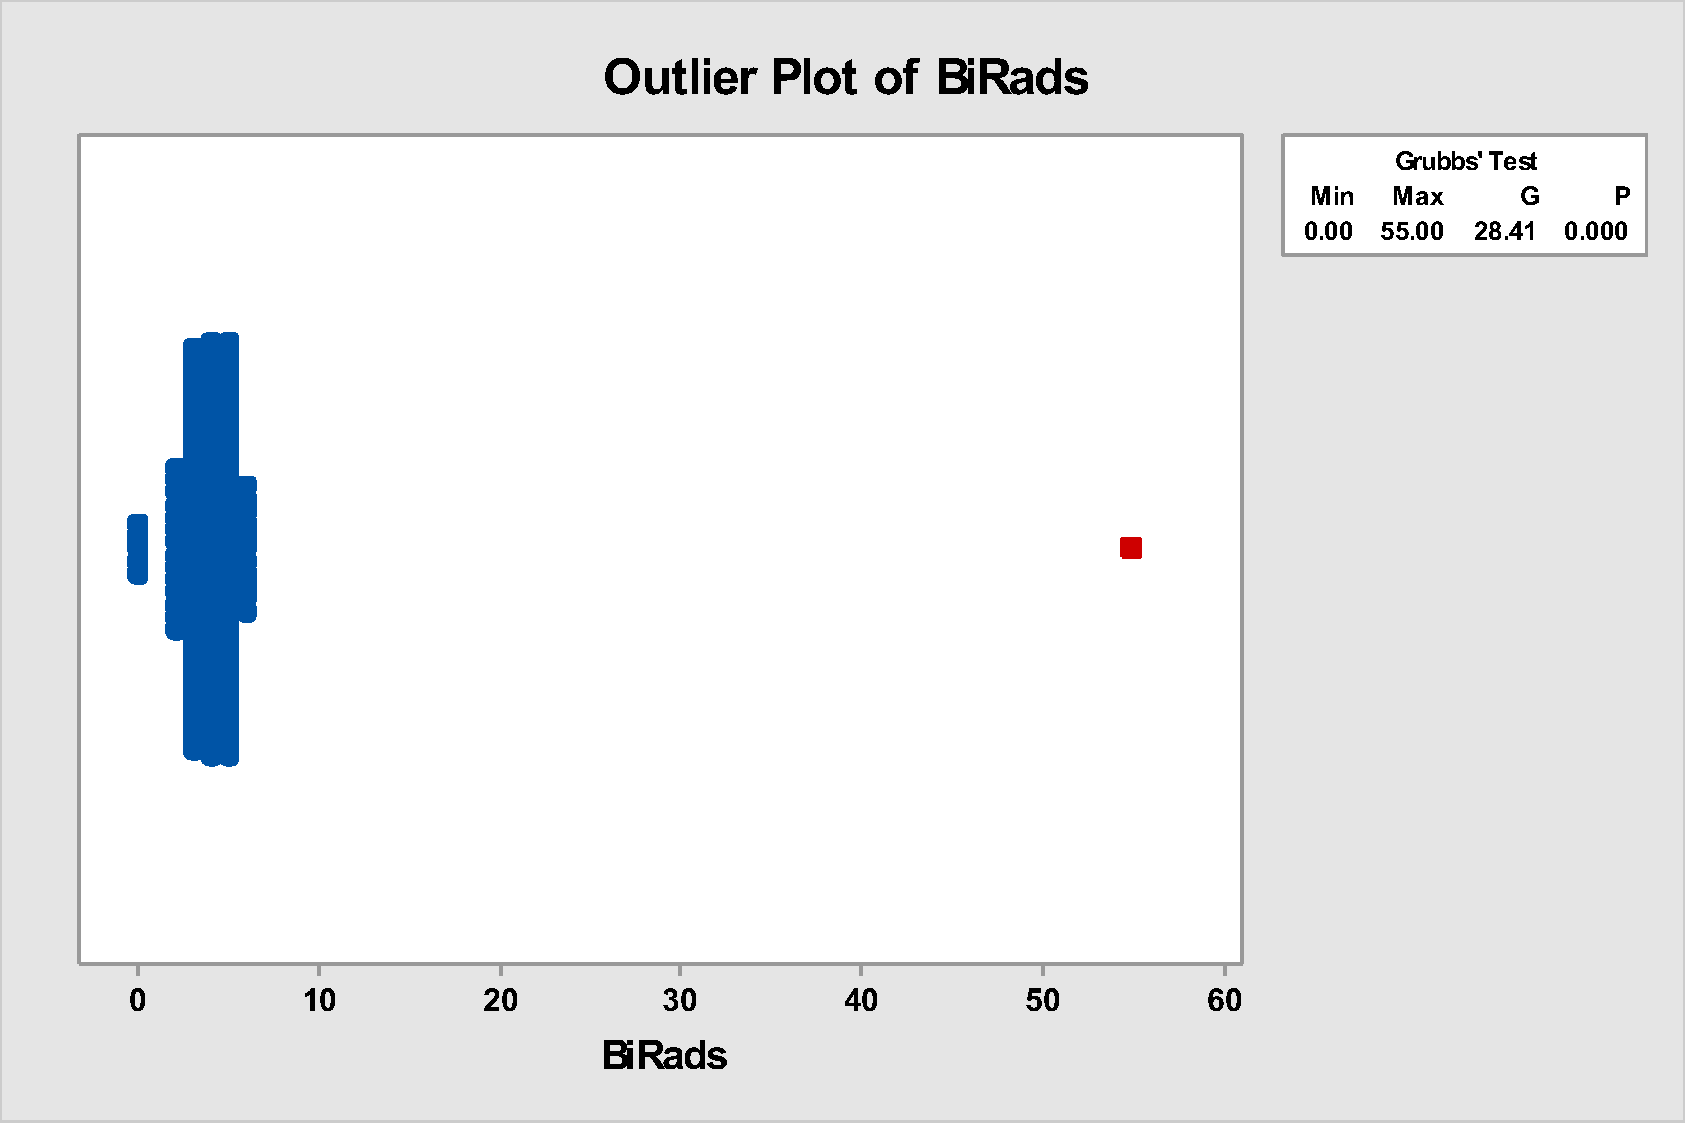
\includegraphics[width=10cm]{birads-outlier-plot}
    \caption{Test}
    \label{fig:Test}
  \end{figure}

% Table generated by Excel2LaTeX from sheet 'Sheet1'
\begin{table}[htbp]
  \centering
  \caption{Confidence (MO=2)}
    \begin{tabular}{c|r}
    \toprule
    \multicolumn{1}{l|}{Confidence} & \multicolumn{1}{l}{Accuracy} \\
    \midrule
    0.05  & 82.2 \\
    0.1   & 82.16 \\
    0.15  & 82.19 \\
    0.2   & 82.27 \\
    0.25  & 82.19 \\
    0.3   & \textbf{82.33} \\
    0.35  & 82.31 \\
    0.4   & 82.12 \\
    \bottomrule
    \end{tabular}%
  \label{tab:addlabel}%
\end{table}%


% Table generated by Excel2LaTeX from sheet 'Sheet1'
\begin{table}[htbp]
  \centering
  \caption{Minimum number of objects highest classification 1 (C=0.3)}
    \begin{tabular}{c|r}
    \toprule
    \multicolumn{1}{l|}{Min Objects} & \multicolumn{1}{l}{Accuracy} \\
    \midrule
    2     & 82.33 \\
    5     & 82.3 \\
    10    & 82.24 \\
    15    & 82.54 \\
    18    & 82.83 \\
    19    & 82.99 \\
    20    & 83 \\
    21    & 83.04 \\
    22    & 82.98 \\
    30    & 83.16 \\
    35    & 83.53 \\
    40    & 83.73 \\
    45    & 83.8 \\
    50    & \textbf{83.82} \\
    60    & 83.04 \\
    70    & 82.82 \\
    \bottomrule
    \end{tabular}%
  \label{tab:addlabel}%
\end{table}%


\begin{table}[htbp]
  \centering
  \caption{Learning rate accuracy from 200-3000 epochs}
    \begin{tabular}{r|rrrrr}
    \toprule
    \multicolumn{1}{r}{} & \multicolumn{5}{|c}{Learning Rate} \\
    & 0.1   & 0.3   & 0.5   & 0.7   & 0.9 \\
    \midrule
        Epochs & \multicolumn{5}{|c}{Accuracy (\%)} \\
    \midrule
    200   & \textbf{81.19} & 80.72 & 80.49 & 80.21 & 79.93 \\
    250   & 80.19 & \textbf{80.99} & 80.58 & 80.39 & 79.97 \\
    350   & 81.27 & \textbf{81.36} & 81.01 & 80.5  & 80.2 \\
    450   & 81.49 & \textbf{81.52} & 80.87 & 80.55 & 80.39 \\
    550   & \textbf{81.72} & 81.56 & 81.13 & 81.08 & 80.74 \\
    650   & \textbf{82.05} & 81.7  & 81.34 & 81.27 & 80.92 \\
    750   & \textbf{82.04} & 81.68 & 81.59 & 81.37 & 81.14 \\
    850   & \textbf{82.16} & 81.77 & 81.76 & 81.52 & 81.16 \\
    950   & \textbf{82.12} & 81.9  & 81.71 & 81.66 & 81.32 \\
    1050  & \textbf{82.13} & 81.96 & 81.84 & 81.77 & 81.28 \\
    1150  & 81.99 & \textbf{82} & 81.8  & 81.81 & 81.34 \\
    1500  & 82.08 & \textbf{82.22} & 81.84 & 81.92 & 81.5 \\
    2000  & 82.23 & \textbf{82.32} & 81.88 & 81.94 & 81.74 \\
    3000  & \textbf{82.25} & 82.24 & 81.84 & 81.86 & 81.69 \\
    \bottomrule
    \end{tabular}%
  \label{tab:addlabel}%
\end{table}%

\begin{table}[htbp]
  \centering
  \caption{Momentum accuracy from 200-3000 epochs (LR=0.4, HL=A)}
    \begin{tabular}{r|rrrrr}
    \toprule
          & \multicolumn{5}{c}{Momentum} \\
    \midrule
    \multicolumn{1}{l|}{Epochs} & 0.1   & 0.3   & 0.5   & 0.7   & 0.9 \\
    \midrule
    200   & 80.59 & \textbf{80.66} & 80.24 & 79.92 & 79.31 \\
    300   & \textbf{81.07} & 80.96 & 80.55 & 80.46 & 79.34 \\
    400   & \textbf{81.31} & 81.17 & 80.68 & 80.55 & 79.49 \\
    500   & 81.33 & \textbf{81.36} & 80.96 & 80.72 & 79.39 \\
    600   & 81.45 & \textbf{81.51} & 81.22 & 80.98 & 79.5 \\
    700   & 81.55 & \textbf{81.64} & 81.38 & 81.15 & 79.48 \\
    800   & 81.52 & \textbf{81.71} & 81.52 & 81.41 & 79.52 \\
    900   & 81.69 & \textbf{81.72} & 81.53 & 81.46 & 79.38 \\
    1000  & \textbf{81.85} & 81.78 & 81.55 & 81.42 & 79.46 \\
    1100  & 81.89 & \textbf{81.98} & 81.61 & 81.63 & 79.66 \\
    1500  & \textbf{82.07} & 82.04 & 81.69 & 81.61 & 79.9 \\
    2000  & \textbf{82.06} & 82.03 & 81.78 & 81.66 & 80.05 \\
    3000  & 81.98 & \textbf{82.05} & 81.81 & 81.64 & 80 \\
    \bottomrule
    \end{tabular}%
  \label{tab:addlabel}%
\end{table}%



\begin{table}[htbp]
  \centering
  \caption{Two hidden layer ANN structure (LR=0.4, M=0.2, E=950)}
    \begin{tabular}{c|rrrrr}
      \toprule
        & \multicolumn{5}{c}{Second Layer Neurons} \\
      \midrule
        \multicolumn{1}{c|}{First Layer Neurons} & 1     & 2     & 3     & 4     & 5 \\
      \midrule
        1 & 82.34 & 82.25 & 82.43 & 82.64 & \textbf{82.67} \\
        2 & 81.78 & 81.89 & 82.29 & 82.06 & \textbf{82.38} \\
        3 & 81.02 & 81.32 & 81.79 & 81.96 & \textbf{82.01} \\
        4 & 80.66 & 81.38 & 80.92 & 80.99 & \textbf{81.07} \\
        5 & 80.55 & 80.53 & \textbf{81.29} & 81.02 & 80.7 \\
      \bottomrule
    \end{tabular}%
  \label{tab:addlabel}%
\end{table}%


\begin{table}[htbp]
  \centering
  \caption{Learning rate impact on accuracy from 250-3000 epochs (M=0.2, HL=1)}
    \begin{tabular}{r|rrrrr}
    \toprule
          & \multicolumn{5}{c}{Learning Rate} \\
    \midrule
    \multicolumn{1}{l|}{Epochs} & 0.1   & 0.3   & 0.5   & 0.7   & 0.9 \\
    \midrule
    250   & 81.73 & \textbf{81.88} & 81.85 & 81.87 & 81.8 \\
    350   & \textbf{82.27} & 82.24 & 82.21 & 82.19 & 82.23 \\
    450   & \textbf{82.58} & 82.49 & 82.39 & 82.33 & 82.35 \\
    550   & 82.55 & \textbf{82.61} & 82.58 & 82.41 & 82.33 \\
    650   & \textbf{82.73} & 82.7  & 82.72 & 82.66 & 82.45 \\
    750   & 82.77 & 82.8  & \textbf{82.83} & 82.74 & 82.5 \\
    850   & 82.79 & \textbf{82.93} & 82.88 & 82.66 & 82.5 \\
    950   & 82.89 & \textbf{83} & 82.87 & 82.78 & 82.55 \\
    1050  & 82.9  & \textbf{83} & 82.89 & 82.83 & 82.61 \\
    1150  & 82.89 & \textbf{83} & 82.87 & 82.88 & 82.69 \\
    1500  & 82.98 & 82.99 & \textbf{83.09} & 83    & 82.87 \\
    2000  & 83.08 & 83.15 & \textbf{83.19} & 83.14 & 83 \\
    3000  & \textbf{83.25} & 83.19 & 83.21 & 83.18 & 83.01 \\
    \bottomrule
    \end{tabular}%
  \label{tab:addlabel}%
\end{table}%



  % • Plan for DT experiments, with justification

  %   (a) Execution of DT experiments to find DT with highest Classification Accuracy

  %   (b) Execution of DT experiments to find the most highly pruned DT that does not have a significantly lower Classification Accuracy than the tree with best CA.

  % • Plan for artificial neural network experiments, with justification

  %   (a) Execution of artificial neural network experiments to find artificial neural network with highest classi- fication accuracy using a single layer of neurons

  %   (b) Execution of artificial neural network experiments to find artificial neural network with highest classi- fication accuracy using a multiple layers of neurons (Individual student judgement to be used on how many layers to be used).


\section{Advanced Pre-processing}
  % • Experiments with different methods of pre-processing the data (scaling, grouping, conversion etc.). This work could contribute marks for work reaching the 86%+ mark band). The section may be omitted if you do not anticipate reaching such a mark.

% http://yatani.jp/HCIstats/PCA
\section{Conclusions}
  % • A description of the best (pruned) decision tree for the dataset (including number of nodes, leaves, pruning parameters etc.).

  % • A diagram of the best pruned decision tree for the dataset.

  % • A description of the best artificial neural network for the dataset (numbers of neurons, layers etc.)

  % • A summary table of best classifiers

  % • A diagram of the best artificial neural network for the dataset.

  % • A statement of which performed best and therefore which you would recommend to the client to solve the task

  % • Short analysis or discussion of results

\newpage

\bibliographystyle{agsm}
\bibliography{report-jim}

\end{document}
